%% Stellarium User Guide

\chapter{Deep-Sky Objects}%\label{deep-sky-objects}
\label{ch:dso}

Extended objects are those which are external to the solar system, and
are not point-sources like stars. These are generally known as
\indexterm{deep-sky objects} or DSO. Extended objects include
galaxies, planetary nebulae and star clusters. These objects may or
may not have images associated with them. Stellarium also comes with a
catalogue with over 14,000 extended objects containing the combined
data from many catalogues, with 190 images.

Since version 0.10.0 Stellarium uses new method of displaying
textures using the ``json'' cataloguing system. At the same time the
Simbad online catalogue was added to the search feature, making the catalog
somewhat redundant and used now only as a first search point or if there
is no internet connection.

If the object has a name (not just a catalogue number), you should add
one or more records to the \file{.../nebulae/default/names.dat} file
(where \file{...} is either the installation directory or the user
directory). See section~\ref{dso:modifyingNamesDat}
\emph{\protect\hyperlink{Modifyingux5fnames.dat}{Modifying names.dat}}
for details of the file format.

If you wish to associate a texture (image) with the object, you must now
add a record to the \file{.../nebulae/default/textures.json} file. See
section~\ref{dso:modTexturesJson} for details of the file format.

Nebula images should have dimensions which are integer powers of two,
i.e. 1, 2, 4, 8, 16, 32, 64, 128, 256, 512, 1024 ... pixels along each
side. If this requirement is not met, your textures may not be visible,
or graphics performance may be seriously impacted. PNG or JPG formats
are both supported.

\section{GUI for managing Deep-Sky Objects}%\label{gui-for-manage-by-deep-sky-objects}
\label{sec:dso:gui}

\begin{figure}[h]
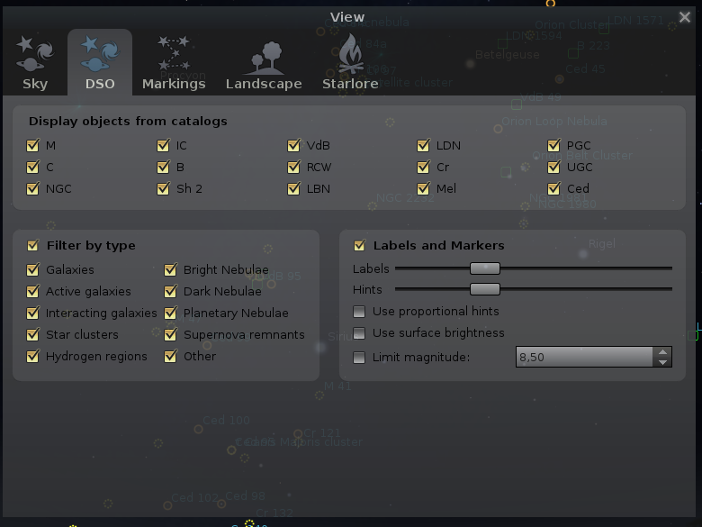
\includegraphics[width=\textwidth]{DSO_GUI}
%\caption{Figure caption}
\end{figure}

\section{Stellarium DSO Catalog}%\label{stellarium-dso-catalog}
\label{sec:dso:catalog}

Stellarium's DSO Catalog contains over 14000 objects and is available
for end users as collection of files:

\begin{itemize}
\item
  \texttt{catalog.txt} - Stellarium DSO Catalog in ASCII format for
  editing data;
\item
  \texttt{catalog.dat} - Stellarium DSO Catalog in binary format for
  usage within Stellarium;
\item
  \texttt{names.dat} - list of proper names of the objects from
  \texttt{catalog.dat} file.
\end{itemize}

ASCII file can be converted into binary format through enabling option
\texttt{devel/convert\_dso\_catalog\ =\ true} in the \texttt{config.ini}
file. The file \texttt{catalog.txt} should be put to the directory
\texttt{.../nebulae/default/}.

Stellarium DSO Catalog contains data and supports the designations for
follow catalogues:

\begin{description}[align=right,labelwidth=2cm]
\item[\textbf{NGC}]  New General Catalogue 
\item[\textbf{IC}] Index Catalogue 
\item[\textbf{M}] Messier Catalog
\item[\textbf{C}] Caldwell Catalogue 
\item[\textbf{B}] Barnard Catalogue 
\item[\textbf{Sh2}] Sharpless Catalogue 
\item[\textbf{VdB}] Van den Bergh Catalogue of reflection nebulae 
\item[\textbf{RCW}]  A catalogue of H$\alpha$-emission regions in the southern Milky Way 
\item[\textbf{LDN}]  Lynds' Catalogue of Dark Nebulae 
\item[\textbf{LBN}]  Lynds' Catalogue of Bright Nebulae 
\item[\textbf{Cr}] Collinder Catalogue 
\item[\textbf{Mel}]  Melotte Catalogue of Deep Sky Objects 
\item[\textbf{PGC}]  HYPERLEDA. I. Catalog of galaxies\footnote{The PGC and UGC catalogues have a partial support}
\item[\textbf{UGC}]  The Uppsala General Catalogue of Galaxies
\item[\textbf{Ced}]  Cederblad Catalog of bright diffuse Galactic nebulae 
\end{description}


\subsection{Modifying catalog.dat}\label{modifying-catalog.dat}

This section is described inner structure of files \texttt{catalog.dat}
(has binary format) and \texttt{catalog.txt} (has ASCII format).
Stellarium can convert ASCII file into the binary format file for usage
within planetarium.

Each line contains one record, each record consisting of the following
fields with \emph{tab} char as delimiter:

\begin{longtabu} to \textwidth {l|l|X}
\toprule
\emph{Column} & \emph{Type} & \emph{Description}\tabularnewline
\midrule
1 & integer & Deep-Sky Object Identificator\tabularnewline
2 & float & RA (decimal degrees)\tabularnewline
3 & float & Dec (decimal degrees)\tabularnewline
4 & float & B magnitude\tabularnewline
5 & float & V magnitude\tabularnewline
6 & string & Object type (Possible values see in table
\emph{\protect\hyperlink{Typesux5fofux5fObjects}{Types of
Objects}}).\tabularnewline
7 & string & Morphological type of object\tabularnewline
8 & float & Major axis size or radius (arcmin)\tabularnewline
9 & float & Minor axis size (arcmin)\tabularnewline
10 & integer & Orientation angle (degrees)\tabularnewline
11 & float & Redshift\tabularnewline
12 & float & Error of redshift\tabularnewline
13 & float & Parallax (mas)\tabularnewline
14 & float & Error of parallax (mas)\tabularnewline
15 & float & Non-redshift distance (Mpc for galaxies, kpc for other
objects)\tabularnewline
16 & float & Error of non-redsift distance (Mpc for galaxies, kpc for
other objects)\tabularnewline
17 & integer & NGC number (New General Catalogue)\tabularnewline
18 & integer & IC number (Index Catalogue)\tabularnewline
19 & integer & M number (Messier Catalog)\tabularnewline
20 & integer & C number (Caldwell Catalogue)\tabularnewline
21 & integer & B number (Barnard Catalogue)\tabularnewline
22 & integer & Sh2 number (Sharpless Catalogue)\tabularnewline
23 & integer & VdB number (Van den Bergh Catalogue of reflection
nebulae)\tabularnewline
24 & integer & RCW number (A catalogue of H$\alpha$-emission regions in the
southern Milky Way)\tabularnewline
25 & integer & LDN number (Lynds' Catalogue of Dark
Nebulae)\tabularnewline
26 & integer & LBN number (Lynds' Catalogue of Bright
Nebulae)\tabularnewline
27 & integer & Cr number (Collinder Catalogue)\tabularnewline
28 & integer & Mel number (Melotte Catalogue of Deep Sky
Objects)\tabularnewline
29 & integer & PGC number (HYPERLEDA. I. Catalog of galaxies);
partial\tabularnewline
30 & integer & UGC number (The Uppsala General Catalogue of Galaxies);
partial\tabularnewline
31 & string & Ced number (Cederblad Catalog of bright diffuse Galactic
nebulae)\tabularnewline
\bottomrule
\end{longtabu}

\subsubsection{Types of Objects}\label{types-of-objects}

Possible values for type of objects in the file \texttt{catalog.dat}.

\begin{longtabu} to \textwidth {l|X}
\toprule
\emph{Type} & \emph{Description}\tabularnewline
\midrule
G & Galaxy\tabularnewline
GX & Galaxy\tabularnewline
AGX & Active Galaxy\tabularnewline
RG & Radio Galaxy\tabularnewline
IG & Interacting Galaxy\tabularnewline
GC & Globular Cluster\tabularnewline
OC & Open Cluster\tabularnewline
NB & Nebula\tabularnewline
PN & Planetary Nebula\tabularnewline
DN & Dark Nebula\tabularnewline
RN & Reflection Nebula\tabularnewline
C+N & Cluster associated with nebulosity\tabularnewline
HII & HII Region\tabularnewline
SNR & Supernova Remnant\tabularnewline
BN & Bipolar Nebula\tabularnewline
EN & Emission Nebula\tabularnewline
SA & Stellar Association\tabularnewline
SC & Star Cloud\tabularnewline
CL & Cluster\tabularnewline
IR & Infra-Red Object\tabularnewline
QSO & Quasar\tabularnewline
Q? & Possible Quasar\tabularnewline
ISM & Interstellar Matter\tabularnewline
EMO & Emission Object\tabularnewline
LIN & LINEAR-type Active Galaxies\tabularnewline
BLL & BL Lac Object\tabularnewline
BLA & Blazar\tabularnewline
MOC & Molecular Cloud\tabularnewline
YSO & Young Stellar Object\tabularnewline
PN? & Possible Planetary Nebula\tabularnewline
PPN & Protoplanetary Nebula\tabularnewline
$\ast$ & Star\tabularnewline
$\ast\ast$ & Double Star\tabularnewline
MUL & Multiple Star\tabularnewline
\emph{empty} & Unknown type, catalog errors, \emph{Unidentified Southern
Objects} etc.\tabularnewline
\bottomrule
\end{longtabu}

\subsection{Modifying names.dat}%\label{modifying-names.dat}
\label{sec:dso:modifyingNamesDat}

Each line in the \file{names.dat} file contains one record. A record
relates an extended object catalogue number (from \file{catalog.dat})
with a name. A single catalogue number may have more than one record in
this file.

The record structure is as follows:

\begin{longtabu} to \textwidth {l|l|l|X}
\toprule
\emph{Offset} & \emph{Length} & \emph{Type} & \emph{Description}\tabularnewline
\midrule
0 & 5 & \%5s & Designator for catalogue (prefix)\tabularnewline
5 & 15 & \%d & Identificator for object in the catalog\tabularnewline
20 & 60 & \%s & Proper name of the object (translatable)\tabularnewline
\bottomrule
\end{longtabu}

If an object has more than one record in the \texttt{names.dat} file,
the last record in the file will be used for the nebula label.

\subsection{Modifying textures.json}%\label{modifying-textures.json}
\label{sec:dso:modifyingTexturesJson}

This file is used to describe each nebula image. The file structure
follows the JSON format, a detailed description of which may be found at
. The textures.json file which ships with Stellarium has the following
structure:

\begin{itemize}
\item
  serverCredits (optional) - a structure containing the following
  key/value pairs:

  \begin{itemize}
  \item
    short - a short identifier of a server where the json file is found,
    e.g. ``ESO''
  \item
    full - a longer description of a server, e.g. ``ESO Online Digitised
    Sky Survey Server''
  \item
    infoURL - a URL pointing at a page with information about the server
  \end{itemize}
\item
  imageCredits - a structure containing the same parts as a
  serverCredits structure but referring to the image data itself
\item
  shortName - an identifier for the set of images, to be used inside
  Stellarium
\item
  minResolution - minimum resolution, applies to all images in the set,
  unless otherwise specified at the image level
\item
  maxBrightness - the maximum brightness of an image, applies to all
  images in the set, unless otherwise specified at the image level
\item
  subTiles - a list of structures describing indiviual image tiles, or
  referring to another json file. Each subTile may contain:

  \begin{itemize}
  \item
    minResolution
  \item
    maxBrightness
  \item
    worldCoords
  \item
    subTiles
  \item
    imageCredits
  \item
    imageUrl
  \item
    textureCoords
  \end{itemize}
\item
  shortName (name for the whole set of images, e.g. ``Nebulae'')
\item
  miniResolution (applies to all images in set)
\item
  alphaBlend (applies to all images in set)
\item
  subTiles list of images. Each image record has the following
  properties:

  \begin{itemize}
  \item
    imageCredits (itself a list of key/pairs)
  \item
    imageUrl (e.g. file name)
  \item
    worldCoords (a list of four pairs of coordinates representing the
    corners of the image)
  \item
    textureCoords (a list of four pairs of corner descriptions. i.e.
    which is top left of image etc)
  \item
    minResolution (over-rides file-level setting)
  \item
    maxBrightness
  \end{itemize}
\end{itemize}

Items enclosed in Quotation marks are strings for use in the program.
Syntax is extremely important. Look at the file with a text editor to
see the format. Items in \textless{}\textgreater{} are user provided
strings and values to suit the texture and source.

\texttt{Line~1~“imageCredits”:~\{“short”~:~“}\texttt{”~:~“infoUrl”:~}\href{http://}{\texttt{http://}}\texttt{\},~}\\
\texttt{Line~2~“imageUrl”~:~“}\texttt{”,~}\\
\texttt{Line~3~“worldCoords”~:~\textless{}~decimal~numerical~values~of~the~J2000~coordinates~of~the~corners~of~the~texture~\textgreater{}~These~values~displayed~to~4~decimal~places~in~the~format~of~the~texture~coordinates~}\\
\texttt{Line~4~“textureCoords”~:~{[}{[}{[}~0,0{]},{[}1,0{]},{[}1,1{]},{[}0,1{]}{]}{]},~Where~0,0~is~South~Left~,~1,0~the~South~Right~,~1,1~North~Right~,~0,1~North~Left~corners~of~texture~Format~=~RA~in~degrees,~Dec~in~degrees~}\\
\texttt{Line~5~“MinResolution”~:~}\texttt{,~}\\
\texttt{Line~6~“maxBrightness”~:~\textless{}~a~numerical~vale~representing~the~absolute~brightness~for~the~display\textgreater{}~}

Calculating of the coords of the corners of the images (plate solving)is
a time consuming project and needs to be fine tuned from the screen
display. As most images will be two dimensional, display on a spherical
display will limit the size to about 1 degree before distortion becomes
evident. Larger displays can be sectioned into a mosaic of smaller
textures for a more accurate display

\section{Adding Extra Nebulae Images}%\label{adding-extra-nebulae-images}
\label{sec:dso:adding_images}

\subsection{\texorpdfstring{Preparing a photo for inclusion to the \file{textures.json} file}{Preparing a photo for inclusion to the textures.json file}}
\label{sec:dso:preparing-a-photo}

\begin{figure}[h]
\centering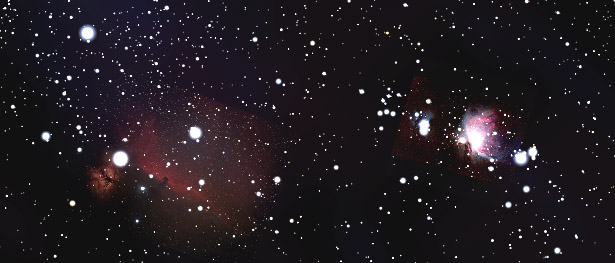
\includegraphics{nebula-display}
\caption{Screen shot of nebula images displayed in Stellarium}
\end{figure}

The first step is to take a photo of the object you wish to display in
Stellarium as a screen backdrop. Then when you have the picture you will
need align it so that north is directly up and not inverted side to side
or up and down as can happen with photos taken with a diagonal mirror in
the path. Next you will need to crop the picture, setting the main
feature at the centre and making the cropped size a factor of $2^n$ eg. 64,
128, 256, 512 or 1024 pixels square. When cropping make sure you leave
at least five prominent background stars.

The next step is to process your photo to make the background
black,black. This will ensure that your background will meld with the
Stellarium background and not be noticed. Suitable programs to do all
this are The Gimp (free in keeping with the Stellarium spirit) or
Photoshop if you can afford it.

When you have your prepared image you will need to plate solve it using
at least 6 known GSC stars that can be identified. That is why the
cropping with plenty of stars was necessary. When the plate is solved
you will need to find the J2000 coordinates of the corners and convert
them to decimal values to form the world coordinates in the
\file{textures.json} file.

\begin{figure}[h]
\centering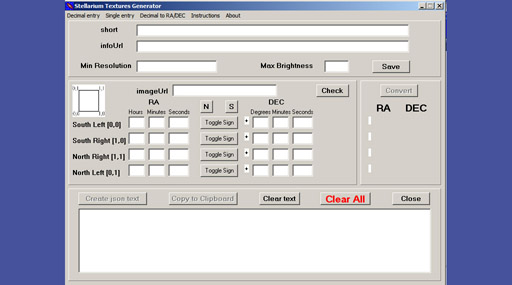
\includegraphics{EQ-Decimal.jpg}
\caption{A program to convert Equatorial coordinates into decimal
form and write a \texttt{textures.json} insert}
\end{figure}

The program in the picture can accept the corner coordinates of a
texture in your plate solving program into decimal values and write an
insert for the \texttt{textures.json} file. It is available as a freebee
from
\url{http://www.madpc.co.uk/~peterv/astroplover/equipnbits/Stellariumtextures.zip}

\begin{figure}[h]
\centering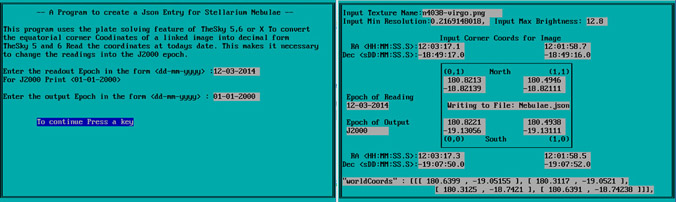
\includegraphics{pix-4.jpg}
\end{figure}

Here is a second program written in Qb64(gl)that will perform the same
task but allows manipulation of the epochs.
\url{http://barry.sarcasmogerdes.com/stellarium/uploads/writejsoninsert.zip}

\subsection{Plate Solving}\label{plate-solving}

Suitable programs that can accept your picture and calculate its corner
coordinates are hard to find. I have only found one that suits our
purpose and it is another expensive planetarium program, TheSkyX Pro.
However the older versions TheSky5 and 6 Pro will also do the job if
suitably configured although I could not solve the test program with the
TheSky6 that uses the same procedure as TheSky5 .

These programs have a link feature that can match your photo to the
selected area of the screen and superimpose it on the display with a box
around your photo provided it can match at least 6 stars from the GSC
that is included with the program. When this is fitted you can read the
corner coordinates of your texture in the Status bar by selecting them
with a mouse. TheSkyX can read these coordinates in J2000 values and
uses textures in the fits format but the earlier programs only read the
coordinates of the current program date. To read the J2000 coordinates
it is necessary to re start the program with the date set to 1-1-2000

To add the picture to TheSky5 you need first make a mono 8 bit version
of the photo and place it on the clipboard. Run TheSky and centre on the
object centre. Look in the Tools menu for the image link and select
setup. Tick show image frame to put a frame around the image.

Paste the clipboard image on the display and use the zoom and position
controls to get it as close to the size and position as possible by
visually matching stars. Go to the menu again and click on link wizard.
If you have been successful the window will show the number of stars
matched and the option to accept or continue. Accept and you will now
see all the matched stars have overlaid the picture. You can now read
off the corner coordinates from the status bar starting at the bottom
(south) left and continuing counter clockwise to the top (north) left.

\subsection{\texorpdfstring{Processing into a \texttt{textures.json}
insert}{Processing into a textures.json insert}}\label{processing-into-a-textures.json-insert}

Place your image in the \texttt{*.png} format in the
\texttt{.../nebulae/default/} folder. Ensure that the name matches the
\texttt{textures.json} entry.

Once you have the corner coordinates of your photo you can add them to
the decimal converter program and it will write an insert
\texttt{nebula.json} as a text file that you can paste directly into the
\texttt{textures.json} file that is in the \texttt{.../nebulae/default/}
folder.

Save the \texttt{textures.json} file with the new insert and run
Stellarium. Select the object in the Object selection window and slew to
it. Your image should be there and with a bit of luck it will nicely
overlay the stars in the Stellarium program. However this only rarely
happens so a little bit of tweaking of the json worldcoords will be
needed to get a perfect match. Select the telescope (equatorial mode).
This will show the area with north up. Select each corner in sequence
and make small changes to the coordinates. Re start Stellarium each time
and check if you have moved the right direction. Continue with each
corner until all the stars match. With a little bit of practice this
will be done in about 10 minutes.


%%% Local Variables: 
%%% mode: latex
%%% TeX-master: "guide"
%%% End: 
